\chapter{Evaluierung von Open API 2.0 Plug-In von OWASP ZAP}
\label{cha:k5}

Die in Abschnitt \ref{ablaufpentest} vorgestellten Schritte eines Penetrationstests werden in diesem Kapitel zur Evaluierung von Open API 2.0 Plug-In von OWASP ZAP herangezogen. Um die bereits entwickelte Springboot Anwendung nach Sicherheitslücken zu testen, werden mit Hilfe des Open API 2.0 Plug-Ins von OWASP ZAP die Penetrationstests durchgeführt.

\section{Ablauf des Open API 2.0 Plug-In von OWASP ZAP}

\subsection{Vorbereitung}

In der Vorbereitungsphase werden die entsprechende Anforderungen für einen Penetrationstest erfüllt, um eine sichere Anwendung zu entwickeln. Hier wird bestimmt, welche Komponente dem Test unterzogen werden. Mittels Springboot kann automatisiert eine Dokumentation der REST API als Swagger 2.0 generiert werden. Die automatisch generierten Restdoc werden in das OpenAPI 2.0 Plug-In von OWASP-ZAP importiert und die geeigneten REST-API-Sicherheitstests für die Schwachstellen durchgeführt. Außerdem kann dieser Penetrationstest in das Konzept des White-Box-Tests eingestuft werden, da vollständige Kenntnisse der zu testenden Infrastruktur vorliegt.

\subsection{Informationsbeschaffung}

Nun, da die Vorbereitungsphase abgeschlossen ist, ist es soweit, mit der Beschaffung von Information über die Springboot Anwendung anzufangen. Diese Springboot Anwendung (Online Shop) enthält bestimmte Produkte. Durch die REST API können Produkte aufgerufen, angezeigt, hinzugefügt, aktualisiert und gelöscht werden. Normalerweiße wird ein Portscan gegen das Zielsystem durchgeführt, um einen Überblick zu bekommen welche Dienste erreichbar sind, aber in dem Fall brauchen wir Portscan nicht, weil automatisch durch das OpenAPI 2.0 Plug-In alle erreichbare Dienste aufgerufen werden können.  Zusätzlich ist zu erwähnen, dass bereits bekannt ist, welche Funktionalitäten diese Springboot-Anwendung besitzt, weshalb in dieser Phase nicht viel Zeit zu investieren ist.

\subsection{Bewertung der Informationen und Risikoanalyse}

In der vorherigen Phase werden alle notwendigen Informationen gesammelt und wird in dieser Phase ausführlich zusammengetragen.
Da ich die Springboot-Anwendung selbst entwickelt habe, wird OWASP-ZAP im  "`Attack Mode"' Penetrationstests durchgeführt und wird auf kein rechtliches Problem gestoßen. Attack Mode bedeutet, dass noch mehr unnötige Informationen in das Programm geladen werden, deshalb ist es wahrscheinlicher das Programm beschädigt und könnte danach vielleicht alle Funktionalitäten nicht erfüllen.

\subsection{Aktive Eindringversuche}

Laut der Risikoanalyse in der dritten Phase können die Penetrationstests für die REST API durchgeführt werden. Durch das OpenAPI 2.0 Plug-In von OWASP ZAP wird in die Springbootanwendung so weit wie möglich vorgedrungen. Da durch den Versuch einzudringen die Springboot-Anwendung beschädigt werden könnten, wird nun eine Schattensystem (eine exakte Kopie des zu testenden Systems) verwendet.\\

\newpage

\begin{figure}[h]
	\centering
	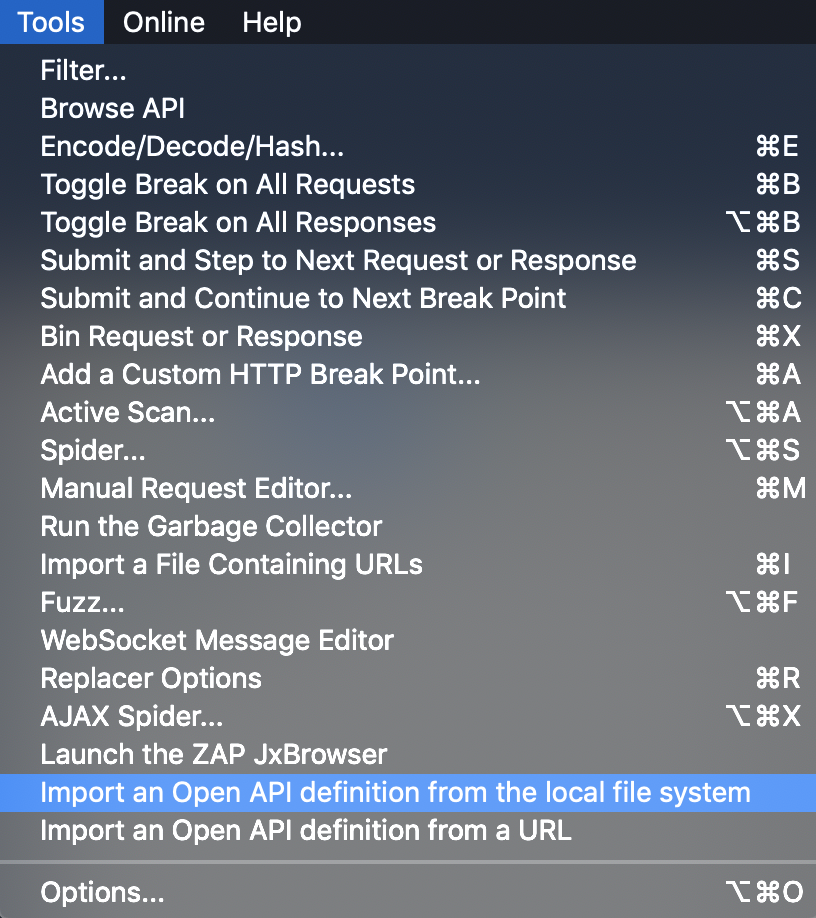
\includegraphics[width=8cm]{2-importbuttonoa2.png}
	\caption{Menuleiste von Open API Plug-In}
	\label{swaggerimport1}
\end{figure}

Um den REST API Penetrationstest durchzuführen, wird von der Menuleiste "`Tools"' geklickt und danach wird "`Import an Open API definition from the local file system"' wie bei der Abbildung \ref{swaggerimport1} gewählt.

\begin{figure}[h]
	\centering
	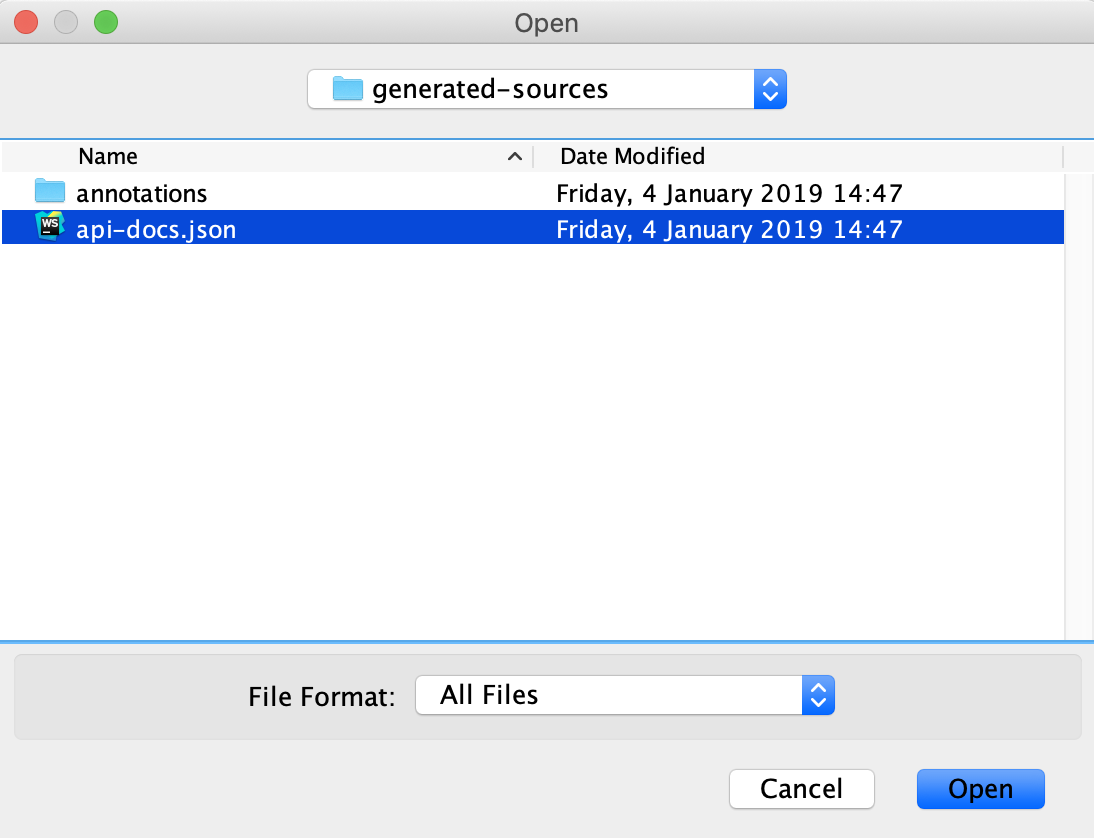
\includegraphics[width=8cm]{3-swaggerfilefortest.png}
	\caption{Importieren von Swagger 2.0 Datei}
	\label{swaggerimport2}
\end{figure}


Wie bei der Abbildung \ref{swaggerimport2} zu sehen, wird lokale Swagger 2.0 Datei ins OWASP ZAP durch das OpenAPI 2.0 Plug-In importiert.

\begin{figure}[h]
	\centering
	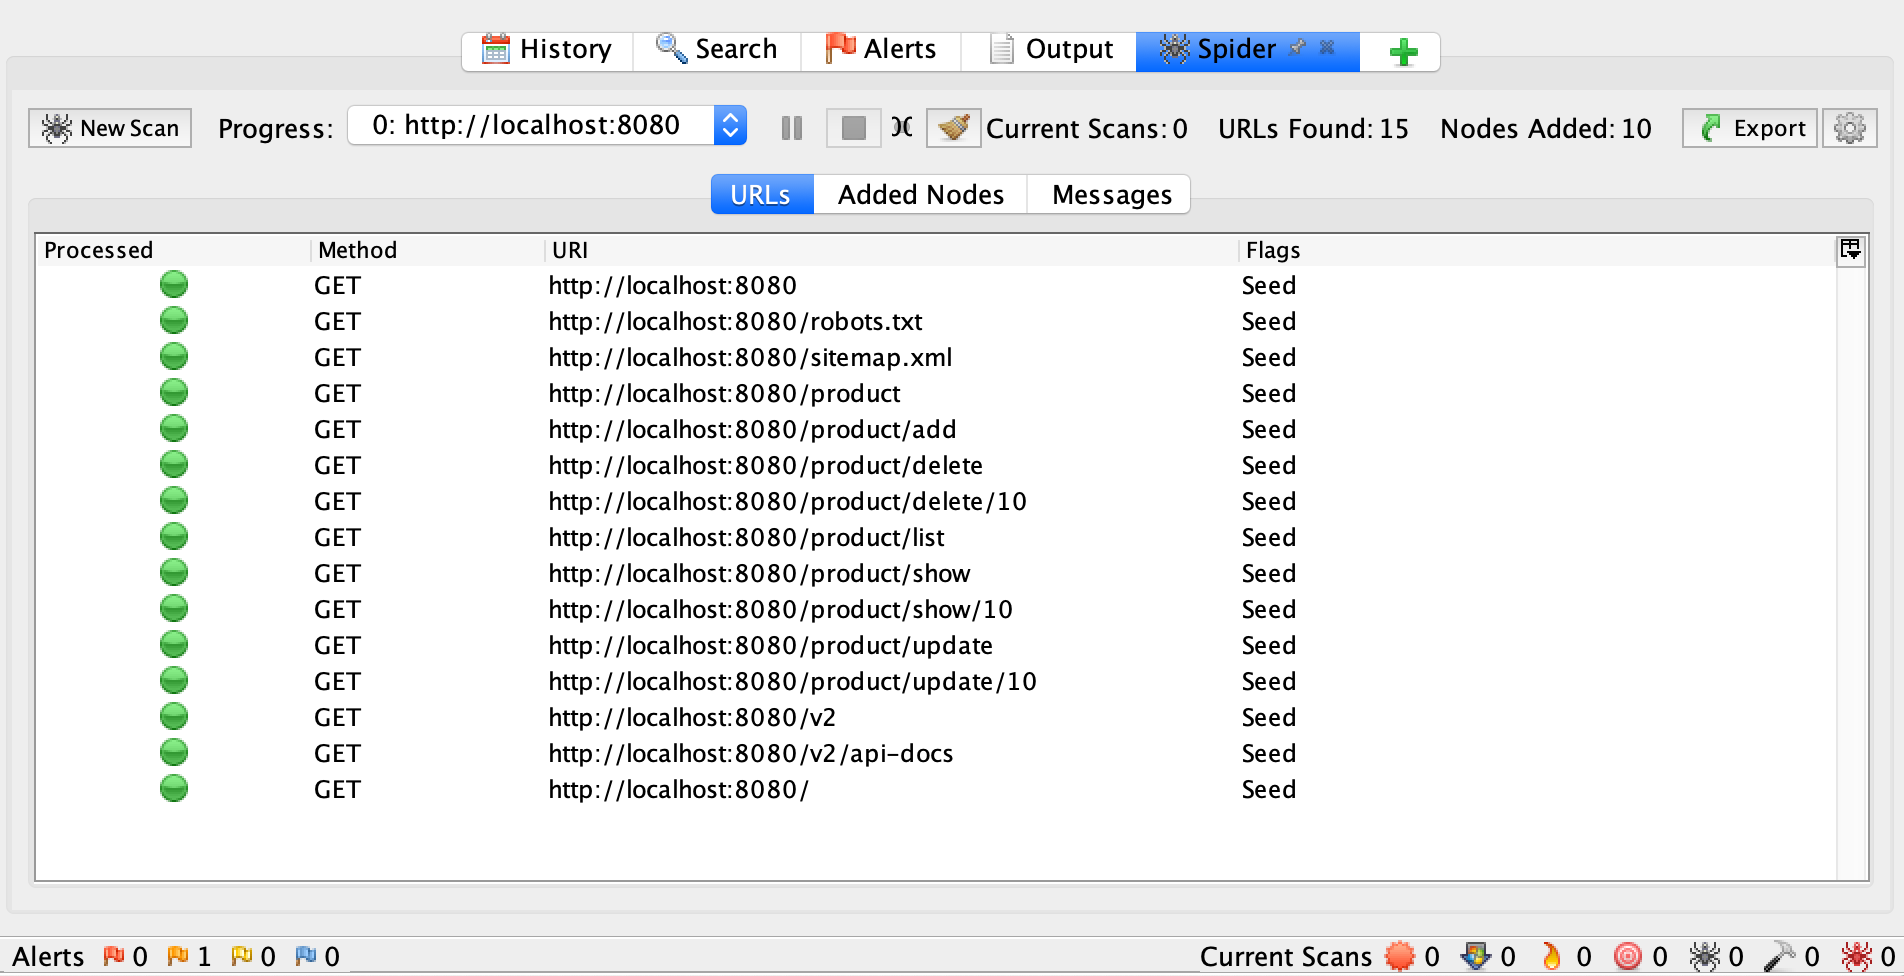
\includegraphics[width=14cm]{5-spiderofurls}
	\caption{Auflistung von erreichbare Diensten}
	\label{swaggerimport3}
\end{figure}

Danach wird durch das Spider alle mögliche Links aufgelistet (siehe \ref{swaggerimport3}), wenn die erreichbar sind. Nun kann mit dem "`Aktive Scan"' wie bei der Abbildung \ref{swaggerimport4} gestartet werden. 

\begin{figure}[h]
	\centering
	\includegraphics[width=14cm]{6-activescancall.png}
	\caption{Aufrufen von Active Scan}
	\label{swaggerimport4}
\end{figure}

Während dem Active Scan-Fortschritt wird unser lokal laufende Springboot-Anwendung für die Sicherheitslücken wie z.B. SQL Injektion, Buffer Overflow, XSS usw. gesucht.

\newpage

Wenn die Suche nach Sicherheitslücken erfolgreich beendet wird, wird alle gefundene Sicherheitslücken wie bei der Abbildung \ref{swaggerimport5} angezeigt.

\begin{figure}[h]
	\centering
	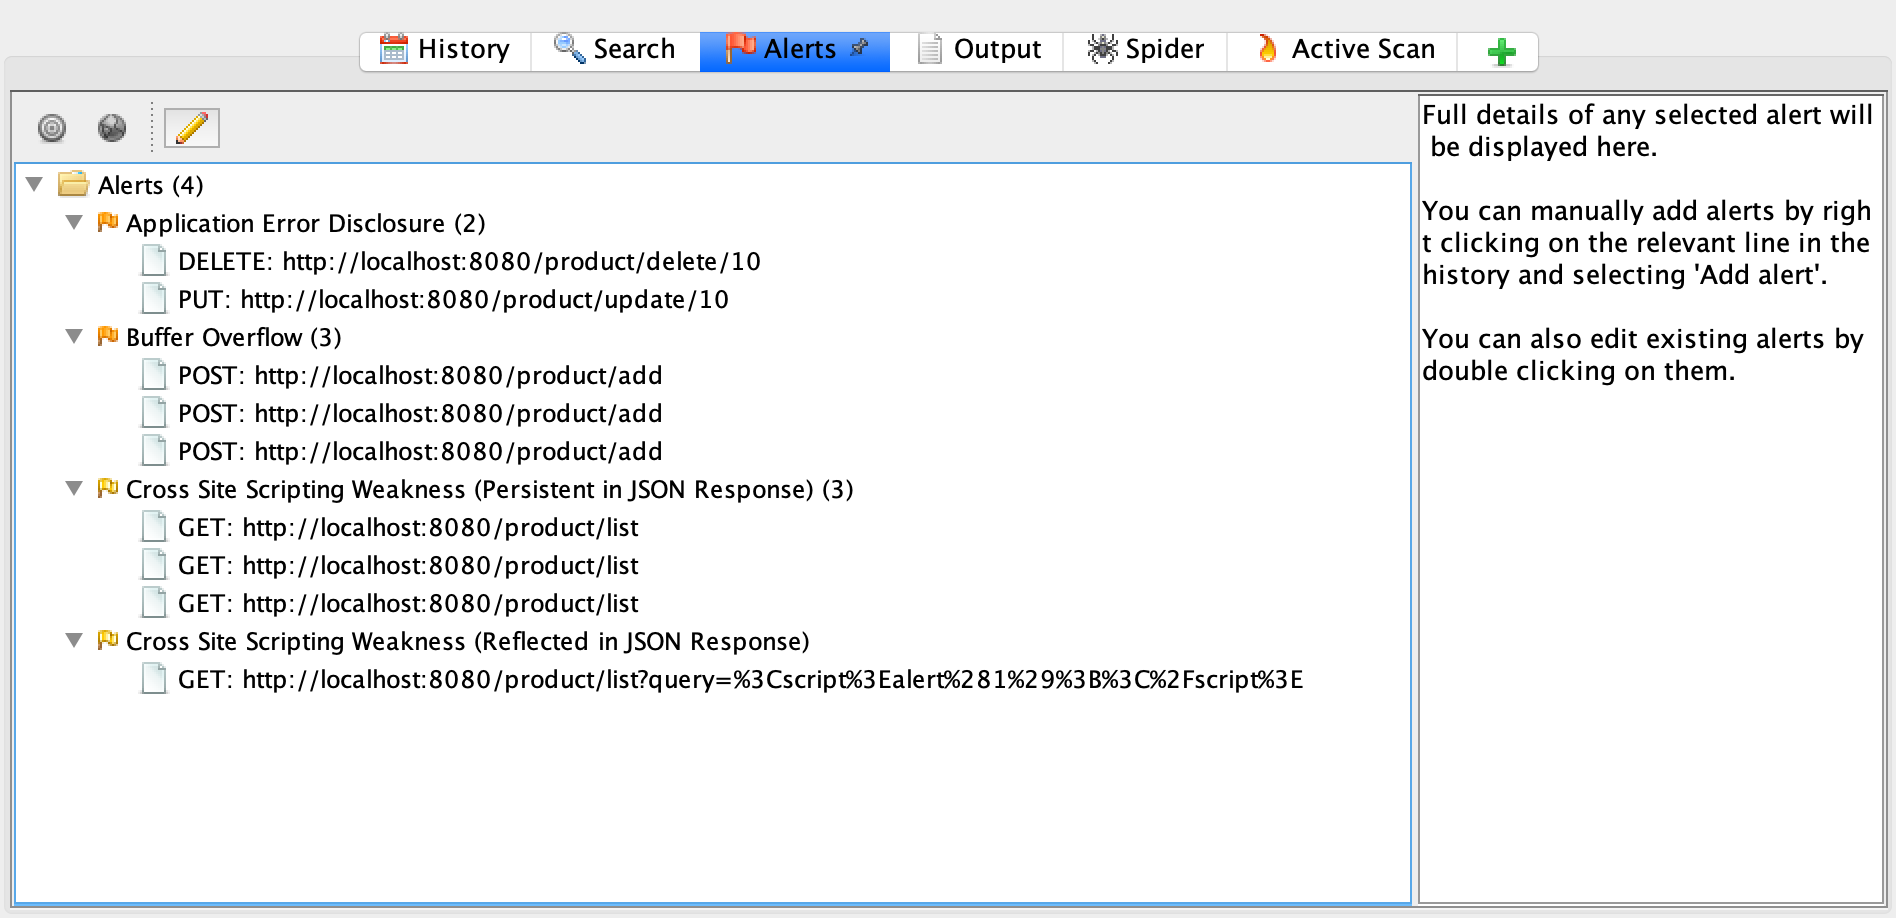
\includegraphics[width=12cm]{7-scanergebnis.png}
	\caption{Ergebnis von Active Scan}
	\label{swaggerimport5}
\end{figure}

\subsection{Abschlussanalyse}

Nach dem Ergebnis des OWASP ZAPs wurden die folgende Sicherheitslücken gefunden;

\begin{itemize}
	\item Application Error Disclosure (2 Stück)
	\item Buffer Overflow (3 Stück)
	\item Cross Site Scripting Weakness (Persistent in JSON Response) (3 Stück)
	\item Cross Site Scripting Weakness (Reflected in JSON Responses)
\end{itemize}

\subsubsection{Vermeidung von Application Error Disclosure}

Wenn eine Anwendung einem Benutzer einen Fehler anzeigt, sollte eine Fehlernachricht die Ursache des Fehlers erklären können. Durch ein normalen Stacktrace kann ein Angreifer zusätzliche Informationen über das System erfahren. 

Zum Beispiel: Wenn ein Benutzer aus Versehen (oder absichtlich) einen \& in einer Inputfeld eingibt, muss die Anwendung anstelle der vollständigen Fehlerdetails einschließlich der Programmierlogik die Meldung "`Fehler aufgrund nicht unterstützter Zeichen. Überprüfen Sie Ihre Eingabe"' anzeigen\cite{ase17}.

\subsubsection{Vermeidung von Buffer Overflow}

asd

\subsubsection{Vermeidung von Cross Site Scripting (Persistent)}

asdasd

\subsubsection{Vermeidung von Cross Site Scripting (Reflected)}

asdasd

\section{restschnittstelle pentestin önemi}

asd
